\documentclass[eikonal.tex]{subfiles}

\begin{document}
  
\section{Implementation of the ordered line integral
  method}\label{sec:implementation}

\begin{figure}
  \centering
  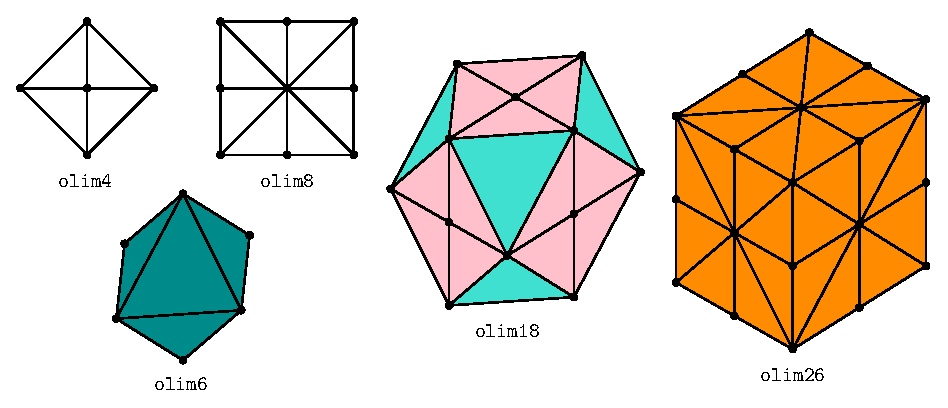
\includegraphics[width=0.95\linewidth]{neighborhoods.eps}
  % \vspace{-1.5em}
  \caption{\emph{Neighborhoods for the top-down family of algorithms.}
    Algorithms \texttt{olim4} and \texttt{olim8} are 2D solvers and
    the rest are 3D solvers. The color coding of tetrahedron updates
    is the same for this figure and \cref{fig:octant-numbering}
    below.}\label{fig:neighborhoods}%
  %\vspace{-1em}
  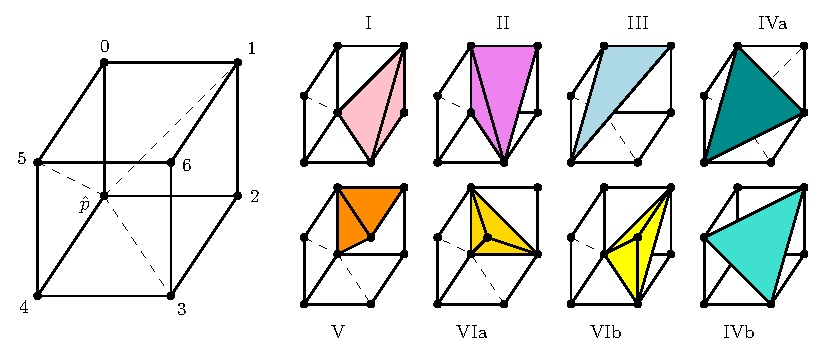
\includegraphics[width=0.95\linewidth]{simplex-groups.eps}
  %\vspace{-1em}
  \caption{\emph{Numbering scheme for update groups for the top-down solvers.} In this
    diagram, $\hat{p}$ is being updated. The diagonally opposite node
    is the sixth (last) node, with the other six nodes numbered 0--5
    cyclically.}\label{fig:octant-numbering}
  \vspace{-0.25em} { \footnotesize
    \begin{tabular}{c|cccccc|cccccc|cccccc|cc}
      0 & $\groupmarker$ & & & & $\groupmarker$ & $\groupmarker$ & $\groupmarker$ & & & $\groupmarker$ & & $\groupmarker$ & $\groupmarker$ & & $\groupmarker$ & & & $\groupmarker$ & $\groupmarker$ & \\
      1 & $\groupmarker$ & $\groupmarker$ & & & & $\groupmarker$ & $\groupmarker$ & $\groupmarker$ & & & $\groupmarker$ & & $\groupmarker$ & $\groupmarker$ & & $\groupmarker$ & & & & $\groupmarker$ \\
      2 & $\groupmarker$ & $\groupmarker$ & $\groupmarker$ & & & & & $\groupmarker$ & $\groupmarker$ & & & $\groupmarker$ & & $\groupmarker$ & $\groupmarker$ & & $\groupmarker$ & & $\groupmarker$ & \\
      3 & & $\groupmarker$ & $\groupmarker$ & $\groupmarker$ & & & $\groupmarker$ & & $\groupmarker$ & $\groupmarker$ & & & & & $\groupmarker$ & $\groupmarker$ & & $\groupmarker$ & & $\groupmarker$ \\
      4 & & & $\groupmarker$ & $\groupmarker$ & $\groupmarker$ & & & $\groupmarker$ & & $\groupmarker$ & $\groupmarker$ & & $\groupmarker$ & & & $\groupmarker$ & $\groupmarker$ & & $\groupmarker$ & \\
      5 & & & & $\groupmarker$ & $\groupmarker$ & $\groupmarker$ & & & $\groupmarker$ & & $\groupmarker$ & $\groupmarker$ & & $\groupmarker$ & & & $\groupmarker$ & $\groupmarker$ & & $\groupmarker$ \\
      \multicolumn{1}{c}{} & \multicolumn{6}{c}{I} & \multicolumn{6}{c}{II} & \multicolumn{6}{c}{III} & \multicolumn{2}{c}{IV}
    \end{tabular}%
    \vspace{1em}
    \begin{tabular}{c|cccccc|cccccc|ccc}
      0 & $\groupmarker$ & & & & & $\groupmarker$ & $\groupmarker$ & & & & $\groupmarker$ & & $\groupmarker$ & & \\
      1 & $\groupmarker$ & $\groupmarker$ & & & & & & $\groupmarker$ & & & & $\groupmarker$ & & $\groupmarker$ & \\
      2 & & $\groupmarker$ & $\groupmarker$ & & & & $\groupmarker$ & & $\groupmarker$ & & & & & & $\groupmarker$ \\
      3 & & & $\groupmarker$ & $\groupmarker$ & & & & $\groupmarker$ & & $\groupmarker$ & & & $\groupmarker$ & & \\
      4 & & & & $\groupmarker$ & $\groupmarker$ & & & & $\groupmarker$ & & $\groupmarker$ & & & $\groupmarker$ & \\
      5 & & & & & $\groupmarker$ & $\groupmarker$ & & & & $\groupmarker$ & & $\groupmarker$ & & & $\groupmarker$ \\
      6 & $\groupmarker$ & $\groupmarker$ & $\groupmarker$ & $\groupmarker$ & $\groupmarker$ & $\groupmarker$ & $\groupmarker$ & $\groupmarker$ & $\groupmarker$ & $\groupmarker$ & $\groupmarker$ & $\groupmarker$ & $\groupmarker$ & $\groupmarker$ & $\groupmarker$ \\
      \multicolumn{1}{c}{} & \multicolumn{6}{c}{V} & \multicolumn{6}{c}{VI} & \multicolumn{3}{c}{VII}
    \end{tabular}%
    \vspace{-0.5em}
  }
  \caption{\emph{Tables of update groups.} These tables should be
    scanned columnwise: each column of dots selects a different
    tetrahedron. Tetrahedra (0, 1, 2), (2, 3, 4), and (4, 5, 0) in
    group I and all tetrahedra in group VII are degenerate and can be
    omitted.}\label{fig:tetrahedra-groups}
\end{figure}

In this section, we describe our ``top-down'' and ``bottom-up''
algorithms. We emphasize the 3D solver, since in 2D, the distinction
between the two is less important. Each algorithm reduces the number
of updates that are done without degrading solution accuracy by using
an efficient enumeration or search of the neighboring simplexes. The
difference between the algorithms is in how this is done.

In \cref{ssec:simplex-enumeration}, we start by showing how to
enumerate update tetrahedra and put them into separate groups of
congruent tetrahedra. By only performing updates from these groups, we
obtain top-down algorithms with stencils of different sizes. Our
numerical tests (\cref{sec:numerical-results}) will show how
neighborhoods of different sizes lead to different patterns of
directional coverage, which can significantly affect the error. We
also discuss the update gaps attainable using these tetrahedron groups
in \cref{ssec:update-gaps}.

Following this, we describe our bottom-up algorithm in
\cref{ssec:bottom-up-search}, which involves first finding the minimal
update of smallest dimension ($d = 0$, a line update), then finding
the minimal update of the next highest dimension ($d = 1$, a triangle
update) which is incident to the original update, and so on. In 3D,
this means finding the minimal line update, doing neighboring triangle
updates which contain the minimal line update, and then neighboring
tetrahedron updates which contain the minimal triangle update. We can
think of this algorithm as a fast search for the first arrival
characteristic.

To minimize the number of updates that are done, it is important to
take advantage of the structure of the underlying constrained
optimization problems that are being solved in order to skip
unnecessary lower or higher dimensional updates. We describe this
procedure in \cref{ssec:algorithms-and-skipping}. How this is done
varies depending on the choice of quadrature rule (\texttt{mp0},
\texttt{mp1}, or \texttt{rhr}) and type of algorithm (top-down or
bottom-up).

\subsection{Simplex enumeration for the top-down
  algorithm}\label{ssec:simplex-enumeration}

When a node is first removed from \texttt{front} and has just become
\texttt{valid} (\cref{enum:get-node}), an isotropic solver must do
updates involving, at the very least, the node's $2n$ von Neumann
neighbors. We can use larger neighborhoods to improve the accuracy of
the result. Doing so does not necessarily improve the order of
convergence of the solver, but can significantly improve the accuracy
of the solution. For all of the solvers considered in this paper, in
3D, we only ever consider neighborhoods with at most 26 neighbors.

For the top-down solver, we simplify things by treating a node's
neighboring octants separately. That is, we iterate over each octant
and do all updates that lie inside that octant before moving onto the
next. To do this, we enumerate all update tetrahedra with vertices
$p \in \{0, 1\}^3$ in a symmetric fashion. Since we assume our update
tetrahedra have been translated so that $\hat{p} = 0 \in \mathbb{Z}^n$
(see \cref{ssec:notation}), this means enumerating
${7 \choose 3} = 35$ choices of vertices. Some choices lead to
degenerate tetrahedra (i.e., such that $p_0, p_1$, and $p_2$ are
linearly dependent), so the number of nondegenerate update tetrahedra
is fewer than 35 per octant. This makes it reasonable to write out the
update procedure as straight-line code.

We enumerate the tetrahedra in a type of ``shift-order'' (see, e.g.,
\cite{arndt2010matters})---that is, we start with an unseen bit
pattern, and group this pattern together with all of its shifts (with
rotation). This groups the tetrahedra into sets that are rotationally
symmetric about the diagonal of the octant. In our implementation, we
conditionally compile different groups so that no unnecessary
branching is done. This is done using C++
templates~\cite{stroustrup2013c++}. Example stencils for the versions
of \texttt{olim6}, \texttt{olim18}, and \texttt{olim26} that are used
for our numerical test are shown in \cref{fig:neighborhoods}. The
tetrahedron groups are shown in
\cref{fig:octant-numbering,fig:tetrahedra-groups}.

\subsection{Update gaps for tetrahedron
  groups}\label{ssec:update-gaps}

If we apply \cref{thm:causality} to the tetrahedron groups enumerated
in \cref{fig:octant-numbering,fig:tetrahedra-groups}, we get the
following update gaps (ignoring the $s^\theta h$ factor):
\vspace{0.5em}
\begin{center}
  \begin{tabular}{lc|lc|lc|lc}
    Group I & $\nicefrac{1}{\sqrt{2}}$ & Group II & $\nicefrac{1}{\sqrt{2}}$ & Group III & $\nicefrac{1}{\sqrt{2}}$ & Group IVa & 0 \\
    \midrule
    Group V & $\nicefrac{1}{\sqrt{3}}$ & Group VIa & 0 & Group VIb & $\boldsymbol{\nicefrac{2}{\sqrt{3}}}$ & Group IVb & $\nicefrac{1}{\sqrt{2}}$
  \end{tabular}
\end{center}
\vspace{0.5em} The idea of the update gap is first explored in
Tsitsiklis's original paper~\cite{tsitsiklis1995efficient}; in this
work, the fact that Group IVa has no update gap and that the update
gap of Group V is $1/\sqrt{3}$ is noted and an $O(N^n)$ algorithm
based on Dial's algorithm is presented using Group V for the update
tetrahedra. This same observation is made in a more recent paper
explicitly detailing a method based on Dial's
algorithm~\cite{kim2001calo}. A method based on a combination of
tetrahedra groups will have as its update gap the minima of each of
the individual groups' update gaps. We note here that a solver based
on a combination of Groups I and VIb has a larger update gap than a
solver based on Group V. This should have a positive impact on the
performance of any parallel Dijkstra-like method.

\subsection{The search procedure used by the bottom-up
  algorithm}\label{ssec:bottom-up-search}

Another approach is to take advantage of the fact that lower
dimensional updates provide some information about the likely
direction of arrival of the first arrival time characteristic. If we
know where the minimum line update is, then the characteristic is
nearby. Starting with the minimum line update, we enumerate
neighboring vertices and perform the corresponding triangle updates,
then enumerate vertices which are sufficiently close to the minimum
triangle update, doing any relevant tetrahedron updates along the way.

While the top-down algorithm is parametrized by the choice of
tetrahedron groups to include, the bottom-up algorithm is parametrized
by the norms used to search for neighboring vertices as well as the
permitted search radii. In 3D, let $p_0$ be the vertex that admits the
minimum line update; then, $p_1$ must satisfy
$\norm{p_1 - p_0}_{q_1} \leq d_1$, where $q_1 = 1, 2$, or $\infty$ and
$d_1$ is a positive integer. Likewise, when searching for tetrahedron
updates, for a candidate vertex $p_2$, we require
$\norm{p_2 - p_1}_{q_2} \leq d_2$ and
$\norm{p_2 - p_0}_{q_2} \leq d_2$ to hold simultaneously.

For our numerical tests, we use the $\ell_1$ norm in both cases
($q_1 = 1 = q_2$), and set $(d_1, d_2) = (1, 2)$ (see
\cref{fig:hu-neighborhoods}). We found this choice of parameters to be
a good compromise between speed and accuracy. Using larger
neighborhoods does lead to a more accurate solution, but causes the
solver to run more slowly. We do not explore the effect of this
parametrization in this paper, since our choice of parameters performs
well enough already (see \cref{sec:numerical-results}).

\begin{figure}[t]
  \centering
  \includegraphics[width=0.85\linewidth]{hu-neighborhoods.eps}
  \caption{\emph{The three types of neighborhoods for the bottom-up
      algorithm with $q_1 = 1 = q_2$, $d_1 = 1$, and $d_2 = 2$.} The
    yellow and blue regions indicate where triangle and tetrahedron
    updates may be performed, respectively. For instance, with $p_0$
    the minimizing line update vertex, candiates for $p_1$ consist of
    the yellow nodes: triangle updates involving these candidates and
    $p_0$ will be performed. Once a yellow node ($p_1$) has been
    selected, tetrahedron updates involving the neighboring blue nodes
    (candidates for $p_2$) will be performed. Note that the updates
    performed correspond roughly to a combination of groups I, V, VIa,
    and VIb.}\label{fig:hu-neighborhoods}
\end{figure}

\subsection{Minimization algorithms and skipping
  updates}\label{ssec:algorithms-and-skipping}

\begin{figure}
  \centering
  \includegraphics[width=0.4\linewidth]{skip-zones.eps}
  \caption{\emph{Skipping lower-dimensional updates when solving the
      unconstrained minimization problem.} For $d = 2$, if
    $\lambda_0^* \in \Delta^2$, all three triangle updates can be
    skipped. On the other hand, when minimizing $F_0$ using
    \cref{thm:f0-exact}, if $\lambda^*_0 \notin \Delta^2$ and
    depending on where $\lambda_0^*$ lies, it is possible to skip one
    or two triangle updates. In this case, we label the different
    regions by the number of updates that it is possible to skip:
    $\lambda^*$ here lies in a region labeled ``2'', since it is
    possible to skip the two triangle updates on the opposite side of
    $\Delta^2$. Along the same lines, if $\lambda^*$ were to lie in a
    region labeled ``1'', two triangle updates would be ``visible'',
    and it would only be possible to skip one
    update.}\label{fig:skip-zones}
\end{figure}

Performing an update is the same as solving
\cref{eq:constrained-minimization} for fixed problem data. When
$F_i = F_0$, we can use \cref{thm:f0-exact} or \cref{thm:equivalence}
to compute $\lambda_0^*$. In this case, $\lambda_0^*$ may lie outside
$\Delta^d$. On the other hand, if $F_i = F_1$, we need to use an
algorithm that can solve the constrained optimization problem defined
by \cref{eq:constrained-minimization}. Our approach has been to use
sequential quadratic programming (SQP), although there are many other
options~\cite{bertsekas1999nonlinear,nocedal2006numerical}. It is
possible to skip some updates; and, indeed, the performance of our
algorithms depends on this happening. We skip updates in three
different ways. The first two strategies for skipping updates are used
by the top-down algorithms, and the third is used by the bottom-up
family of algorithms.

\paragraph{Top-down constrained skipping} When computing an update
using a constrained solver, we can rule out all incident
lower-dimensional updates, since we have computed the global
constrained optimum on $\Delta^d$.

\paragraph{Top-down unconstrained skipping} If we do an update using
an unconstrained solver, then depending on where the optimum
$\lambda_0^*$ lies, we can skip some lower-dimensional updates. The
idea is simple: since $F_0$ is strictly convex, if we consider a
straight line starting at $\lambda_0^*$ and extending in some
direction, then $f$ restricted to that line is monotonically
increasing as we move away from $\lambda_0^*$. Hence, for a
tetrahedron update, if $\lambda_0^* \notin \Delta^2$, then we can skip
all updates which are not ``visible'' (in parameter space) from
$\lambda_0^*$. This is illustrated in the \cref{fig:skip-zones}.

\paragraph{Bottom-up KKT skipping} We can also skip higher-dimensional
updates. For example, if we do the three triangle updates on the
boundary of a tetrahedron update, we can use the Karush-Kuhn-Tucker
necessary conditions for optimality of a constrained optimization
problem~\cite{nocedal2006numerical} to determine if the minimizer on
the boundary is also a global minimizer for the constrained
minimization problem given by \cref{eq:constrained-minimization}. Let
$L(\lambda, \mu) = F_i(\lambda) + (A\lambda - b)^\top \mu$ be the
Lagrangian function, where $\mu \in \mathbb{R}^{d + 1}$ is the vector
of Lagrange multipliers. Since $F_0$ is strictly convex and since we
assume $h$ is small enough for $F_1$ to be strictly convex, if
$\lambda^*$ lies on the boundary of $\Delta^d$, we only need to check
that the optimum Lagrange multipliers $\mu^*$ are dual feasible; i.e.,
whether
$\mu^* \geq 0$~\cite{bertsekas1999nonlinear,nocedal2006numerical}. For
$\lambda^* \in \partial \Delta^d$, letting
$\mathcal{I} = \set{i : (A\lambda - b)_i = 0}$ be the set of active
constraints' indices, stationarity requires:
\begin{equation}\label{eq:stationarity}
  A^\top_{\mathcal{I}} \mu_{\mathcal{I}}^* = \nabla F_i(\lambda).
\end{equation}
See \cref{eq:Delta-LMI} for the definition of $A$; the notation
$A_{\mathcal{I}}$ refers to the submatrix consisting of rows of $A$
indexed by $\mathcal{I}$. For a tetrahedron update in 3D,
$A \in \mathbb{R}^{3 \times 2}$ and $|\mathcal{I}| \leq 2$ (not all
three constraints be active simultaneously). In particular, if
$i \notin \mathcal{I}$, then $\mu_i^* = 0$, and otherwise, $\mu_i^*$
can be computed easily from \cref{eq:stationarity}. Once the full
vector of Lagrange multipliers has been computed, if $\mu^* \geq 0$,
then the update may be skipped. A modified version of this strategy
for skipping updates was used in our work on computing the
quasipotential for nongradient SDEs in 3D~\cite{yang2019computing}.

\subsection{The top-down and bottom-up algorithms}

To describe our top-down algorithm, we define:
\begin{equation}\label{eq:calU}
  \begin{aligned}
    \calV_d = \big\{\set{p_0, \hdots, p_d}: \; &p_i\texttt{.state}=\texttt{valid} \mbox{ for } i = 0, \hdots, d, \\
    &\mbox{and } \set{p_0, \hdots, p_d} \mbox{ belongs to the selected update group}, \\
    &\mbox{and } \pnew \in \set{p_0, \hdots, p_d} \big\}
  \end{aligned}
\end{equation}
for $d = 0, \hdots, n - 1$. These sets collect all possible simplex
updates: i.e., updates which both belong to a group as defined in
\cref{ssec:simplex-enumeration} and are \texttt{valid}. The third
condition is an important optimization. To see why it is correct, fix
an update set $\calV_d$. If $\set{p_0, \hdots, p_d}$ satisfies the
first two conditions but not the third, we can see that $\hat{p}$
would have already been updated from it in a previous iteration. All
new information affecting $\hat{U}$ during this iteration must be
computed from an update involving $\pnew$.

\begin{algorithm}[H]
  \caption{The top-down hierarchical algorithm for computing
    $U(\hat{p})$ (\cref{enum:update-U} of
    \cref{alg:dijkstra-like}).}\label{alg:top-down}
  \textbf{Input:} the neighboring update points $(p_0, \hdots, p_d)$,
  and, for $i = 0, \hdots, d$, the downwind solution value
  $U_i = U(p_i)$ and the slowness $s_i = s(p_i)$. \\
  \textbf{Output:} a new solution value $\hat{U} = U(\hat{p})$, where
  $\hat{U} > U_i$ for $i = 0, \hdots, d$.
  \begin{enumerate}[nolistsep]
  \item Set $\hat{U} \gets \infty$.
  \item Initialize $\calV_d$ according to \cref{eq:calU} for each
    $d = 0, \hdots, n - 1$.
  \item For $d = n - 1$ down to $0$:
    \begin{enumerate}
    \item For each $(p_0, \hdots, p_d) \in \calV_d$:
      \begin{enumerate}
      \item If $F_i = F_0$ (\texttt{mp0} or \texttt{rhr}):
        \begin{enumerate}
        \item Compute $U$ for $(p_0, \hdots, p_{d})$ using
          \cref{thm:f0-exact} or \cref{thm:equivalence}.
        \item Remove updates from $\calV_0, \hdots, \calV_{d-1}$ by
          visibility (see \cref{fig:skip-zones}).
        \end{enumerate}
      \item Otherwise, if $F_i = F_1$ (\texttt{mp1}):
        \begin{enumerate}
        \item Compute $U$ by solving
          \cref{eq:constrained-minimization} numerically (we use SQP).
        \item Remove all lower-dimensional updates from
          $\calV_0, \hdots, \calV_{d-1}$.
        \end{enumerate}
      \item Set $\hat{U} \gets \min(\hat{U}, U)$.
      \end{enumerate}
    \end{enumerate}
  \end{enumerate}
\end{algorithm}

The bottom-up algorithm builds up each update $(p_0, \hdots, p_d)$ one
vector at a time by searching for adjacent minimizing updates of
higher dimension. The optimization involving $\pnew$ described above
can be incorporated by initially setting $p_0 \gets \pnew$.

\begin{algorithm}[H]
  \caption{The bottom-up hierarchical algorithm for computing
    $U(\hat{p})$ (\cref{enum:update-U} of
    \cref{alg:dijkstra-like}).}\label{alg:bottom-up}
  \textbf{Input:} for $i = 0, \hdots, d$, the update point $p_i$, the
  values
  $U_i = U(p_i)$, and $s_i = s(p_i)$. \\
  \textbf{Output:} the new solution value $\hat{U} = U(\hat{p})$.
  \begin{enumerate}[nolistsep]
  \item Set $\hat{U} \gets \infty$ and $p_0 \gets \pnew$.
  \item For $i = 1, \hdots, n - 1$:
    \begin{enumerate}
    \item For each \texttt{valid} $p_i$ close enough to
      $p_0, \hdots, p_{i-1}$ (see \cref{ssec:bottom-up-search}), do
      the update corresponding to $(p_0, \hdots, p_i)$ and keep track
      of the minimizing $\lambda^* \in \Delta^i$. This update can
      optionally be skipped by first computing $\mu^*$ corresponding
      to the optimum of the incident lower-dimensional update
      $(p_0, \hdots, p_{i-1})$ and checking if
      $\mu^* \geq 0$.\label{item:bottom-up-for}
    \item Let $p_i$ be the node which forms the update with the
      minimum value.
    \item If $F_i = F_0$ (\texttt{mp0} or \texttt{rhr}), compute $U$
      for $(p_0, \hdots, p_{i})$ using \cref{thm:f0-exact} or
      \cref{thm:equivalence}.
    \item Otherwise, if $F_i = F_1$ (\texttt{mp1}), compute $U$ for
      $(p_0, \hdots, p_{i})$ by solving
      \cref{eq:constrained-minimization}.
    \item Set $\hat{U} \gets \min(\hat{U}, U)$.
    \end{enumerate}
  \end{enumerate}
\end{algorithm}

\end{document}

%%% Local Variables:
%%% mode: latex
%%% TeX-master: "sisc-eikonal.tex"
%%% End:
